
\documentclass[oneside]{ausarbeitung}
\bibliography{latexlit}


% ----------------------------------------------------------------------

\begin{document}

%--- Sprachauswahl
% Erlaubte Werte:
%   \selectlanguage{english}
%   \selectlanguage{ngerman}
\selectlanguage{english}

%--- Art der Arbeit
% Erlaubte Werte:
%   \Praxissemesterbericht
%   \Projektbericht
%   \Bachelorarbeit
\Seminararbeit
%   \Masterarbeit

%--- Studiengang:
% Erlaubte Werte:
%   \Informatik
%   \Elektronik
%   \DataScience
\Informatik

\title{Algorithmic Game Theory}

\author{Tim Staudenmaier}
\matrikelnr{75981}

%--- Ist der Erstbetreuer (\examinerA) an der Hochschule ein Professor?
% Erlaubte Werte:
%   \examinerIsAProfessortrue   % Ja
%   \examinerIsAProfessorfalse  % Nein
\examinerIsAProfessortrue   % Ja

%--- Betreuer
\examinerA{Prof.~Dr.~Thomas~Thierauf}
%\examinerB{Prof.~Dr.~Ulrich~Klauck}

%--- Einreichungsdatum
\date{14.3.2023}

%--- Angaben zur Firma
% Auskommentieren, wenn die Arbeit nicht bei einer ext. Firma gemacht wurde.
%\companyname{Beispielfirma}
%\industrialsector{Beispielbranche}
%\department{Beispielabteilung}
%\companystreet{Beispielstr. 1}
%\companycity{12345 Musterstadt}

%--- Angaben zum Betreuer bei dieser Firma
%\advisorname{Name des Betreuers}
%\advisorphone{(01234) 567-890}
%\advisoremail{name@company.xxx}

%--- Titelseite Anzeigen
\maketitle
\cleardoublepage

%---
\pagenumbering{roman}
\setcounter{page}{1}

%--- Firmendaten Anzeigen
% Auskommentieren, wenn die Arbeit nicht bei einer ext. Firma gemacht wurde.
%\makeworkplace
%\cleardoublepage

%--- Eidesstattliche Erklärung anzeigen
\makeaffirmation
\cleardoublepage

%---
\begin{abstract}
  This work serves as an introduction to the topic of Algorithmic Game Theory. The basic principles and applications of Algorithmic Game Theory are explained and discussed. Some basic examples of Algorithmic Game Theory are presented, including popular games and dilemmas, like the Prisoner's Dilemma. Different groups of games, such as coordination games or cooperative games, are introduced and their optimal strategies and differences are outlined.

 The different types of optimal and stable solutions, called Nash equilibria, are presented. If a solution is a Nash equilibrium, none of the players can improve their outcome of the game by changing the choices they made. The requirements and characteristics of these Nash Equilibria are explained and ways to compute them are discussed. The complexity of these computations and possible solutions are outlined. The Lemke-Howson algorithm for calculating Nash equilibria is explained and the PPAD-completeness of Nash is discussed.

 An outlook on current research in the field of Algorithmic Game Theory is given and the importance of Algorithmic Game Theory in today's world is discussed.
\end{abstract}
%-----------------------------------------------------------------------
\cleardoublepage
\tableofcontents

%---
\listoffigures

%---


\cleardoublepage
\pagenumbering{arabic}
\setcounter{page}{1}

\algrenewcommand\algorithmicrequire{\textbf{Input:}}
\algrenewcommand\algorithmicensure{\textbf{Output:}}

% ----------------------------------------------------------------------

% \chapter{Network Generation}
% \label{cha:network_generation}
% The developed tool provides a user interface for generating networks to simulate epidemics. To create these networks, different groups of people can be defined. Each group consists of $n$ nodes, the members, each of which has a certain number of edges to other nodes of the same group. The number of edges per node is determined by a mean $\mu$ and a delta $\delta$. Each node will then have an edge count between $\mu - \delta$ and $\mu + \delta$.

Let $g1$ and $g2$ be two different groups. Then in addition to the above mentioned edges within a group, it is also possible to specify the number of edges between the nodes of the two groups with an average and delta value, in the same way as described above.

To create a network graph that meets all of these requirements multiple algorithms are needed.

\section{Creating edges within a group}
\label{sec:creating_edges_in_group}
Let $g$ be a group of $n$ nodes, each of which needs between $\mu - \delta$ and $\mu + \delta$ edges. Then the first step is to generate a sequence of $n$ integer numbers within this range. This sequence represents the degree each node should have at the end.

\subsection{Randomly adding new edges}
\begin{algorithm}
\caption{Adding random edges}
\label{alg:random_edges}
\begin{algorithmic}
\State $nodes \gets $nodes with less than required degree
\While{$nodes$ is not empty}
    \State $n1, n2 \gets$ two unconnected nodes
    \State connect $n1$ and $n2$
    \If {$n1$ has required degree}
        \State remove $n1$ from $nodes$
    \EndIf
    \If {$n2$ has required degree}
        \State remove $n2$ from $nodes$
    \EndIf
\EndWhile
\end{algorithmic}
\end{algorithm}

This algorithm was the first iteration for creating the networks, it has two issues. 
\newline

First, not every sequence of degrees is graphic, e.g. not every sequence of degrees has a corresponding simple graph. A simple graph is a graph consisting only of undirected edges and no loops.

For example, let $s$ be a sequence of random integers with sum $m$. If $m$ is not even, $s$ is definitely not graphic, because in a simple graph without loops, every edge increases the total degree of all nodes by two. Thus it is impossible to have a total degree of all nodes that is not even. This is not checked in the above algorithm \ref{alg:random_edges}, which would cause the $nodes$ list to contain only one node at the end, making it impossible to select two unconnected nodes from it.
\newline

The second issue is that by adding edges randomly it is possible to end up in a situation, where all remaining edges are already connected but have still not reached the required degree.

\begin{figure}
    \centering
    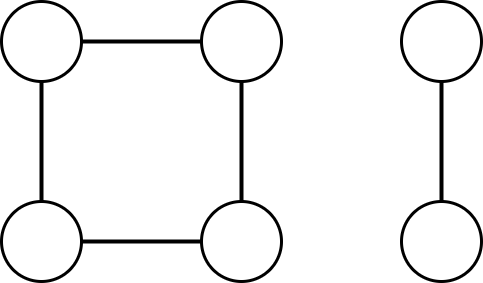
\includegraphics[width=0.5\linewidth]{images/impossible_graph.png}
    \caption{Graph created by random algorithm \ref{alg:random_edges} with $\mu=2$ and $\delta=0$}
    \label{fig:impossible_graph}
\end{figure}

Figure \ref{fig:impossible_graph} shows one such situation. In this graph each node needs to have a degree of exactly two. In theory it is possible to create such a graph, but the random algorithm \ref{alg:random_edges} may end up in the situation shown in the figure. Here the only two nodes remaining in the $nodes$ list are the two on the right which are already connected. From this state it is impossible to create a graph that satisfies the degree requirements.
\newline

The second iteration of the algorithm uses a more methodical approach to adding the edges to solve the above issues.

\subsection{Erdos-Gallai Theorem}
To solve the first problem of degree sequences that are not graphic, the Erdos-Gallai Theorem is used. It provides one of the two known approaches to solving the graph realization problem, i.e. it gives a necessary and sufficient condition for a finite sequence of natural numbers to be the degree sequence of a simple graph.

\begin{equation}
\sum_{i=1}^{k} d_i \leq k(k-1) + \sum_{i=k+1}^{n} \min(k, d_i)
\end{equation}
for all integers \(k\) with \(1 \leq k \leq n\), where \(d_1 \geq d_2 \geq \ldots \geq d_n\) are non-negative integers.

A sequence of degrees is graphic if and only if \(d_1 + d_2 + \ldots + d_n\) is even and the above equation holds for every $k$. The inequality ensures that the sum of the first $k$ terms of the degree sequence does not exceed the theoretical maximum number of edges $(k(k-1))$ plus the sum of the remaining edges $\sum_{i=k+1}^{n} \min(k, d_i)$ for the remaining vertices.

For this tool, every degree sequence needs to be graphic, because it should always be possible to generate a graph for the user's input. This means that if the Erdos-Gallai Theorem shows that a sequence is not graphic, it must be changed until it is. This is done by simply decrementing a random number of the degree sequence by one.

If the Erdos-Gallai Theorem failed because the sum was not even, the sum will be even after decrementing once. By decrementing random numbers of the sequence, only the left side of the inequality gets smaller, because $k$ never changes. This means after decrementing enough times, the theorem will always be fulfilled. Thus, any sequence of degrees can be changed to be graphic.

The python implementation of this algorithm can be seen in \ref{lst:erdos_gallai}.

\begin{lstlisting}[language=python, caption={Erdos-Gallai Theorem in Python}, label={lst:erdos_gallai}]
def _erdos_gallai(self) -> bool:
    if sum(self.deg_seq) % 2 != 0:
        return False
    n = self.size
    for k in range(1, n + 1):
        if sum(self.deg_seq[:k]) > k * (k - 1) + sum(min(k, d) for d in self.deg_seq[k + 1 :]):
            return False
    return True
\end{lstlisting}

\subsection{Havel-Hakimi algorithm}
\label{sub:havel_hakimi}
After creating a graphic degree sequence using the Erdos-Gallai Theorem, with all degrees within the $\mu - \delta$ and $\mu + \delta$ range, this degree sequence needs to be converted to a network graph.

\begin{algorithm}
\caption{Havel-Hakimi algorithm}
\label{alg:havel_hakimi}
\begin{algorithmic}
\State $deg\_seq \gets $ graphic sequence of degrees
\State $nodes \gets $ list of nodes, with same length as $deg\_seq$
\While{$sum(deg\_seq) > 0$}
    \State $n \gets nodes.pop(0)$
    \State $d \gets deq\_seq.pop(0)$
    \State $targets \gets $ n nodes with highest degree from $nodes$
    \For{$t$ in $targets$}
        \State connect $t$ and $n$
        \State $deg\_seq[t] \gets deg\_seq[t] - 1$
    \EndFor
\EndWhile
\end{algorithmic}
\end{algorithm}

Using the Havel-Hakimi algorithm \ref{alg:havel_hakimi} a simple graph can be constructed for every graphic sequence of degrees. This algorithm always finds a correct solution as proven by Erdős et al. \cite{havelHakimi}.

\subsubsection{Python implementation}
The Havel-Hakimi algorithm is implemented in the class HavelHakimi. This class has properties for the sequence of degrees \texttt{deg\_seq}, list of node ids \texttt{node\_id\_seq} and a dictionary which nodes are connected \texttt{edges} (each key node id has an undirected edge to all its value node ids).

First the \texttt{node\_id\_seq} is sorted to be non-increasing and the \texttt{node\_id\_seq} is shuffled to assign random degrees to each node. Then the Havel-Hakimi algorithm is used:

\begin{lstlisting}[language=python, caption={Havel Hakimi Algorithm in Python}, label={lst:havel_hakimi}]
def _connect_nodes(self):
    while sum(self.deg_seq) > 0:
        node = self.node_id_seq.pop(0)
        deg = self.deg_seq.pop(0)
        targets = self._get_highest_n_nodes(deg)
        for target in targets:
            self.deg_seq[self.node_id_seq.index(target)] -= 1
        self.edges[node] = targets
        self._sort_sequence()
\end{lstlisting}

The function in listing \ref{lst:havel_hakimi} implements the above algorithm \ref{alg:havel_hakimi}. After each iteration, the degree sequence is sorted so it is non-increasing again. When sorting the \texttt{deg\_seq} it is important that the \texttt{node\_id\_seq} is altered in the same way so each node id still corresponds to the same degree, this function is shown in \ref{lst:sorting}.

\begin{lstlisting}[language=python, caption={Sorting degrees and node ids}, label={lst:sorting}]
def _sort_sequence(self):
    self.node_id_seq = [x for _, x in sorted(zip(self.deg_seq, self.node_id_seq), reverse=True)]
    self.deg_seq.sort(reverse=True)
\end{lstlisting}

\section{Creating edges between groups}
Randomly creating edges between two groups leads to similar problems as described in section \ref{sec:creating_edges_in_group}. Therefore, a modified version of the Havel-Hakimi algorithm and the Erdos-Gallai theorem is used.

\subsection{Creating the degree sequence}
Let $g1$ and $g2$ be two disjoint groups of size $n$ and $m$. If $n \neq m$, it may not be possible for every node to have a degree between $\mu - \delta$ and $\mu + \delta$. Let $n = 5$ and $m = 10$ with $\mu = 5$, $\delta = 0$. If every node in $g2$ has a degree of $5$, all nodes in $g1$ would have a degree of $10$. If every node in $g1$ has a degree of $5$, the average degree of the nodes in $g2$ would be only $2.5$.

So if $n \neq m$ one group may have lower degrees than the minimum or higher degrees than the maximum for certain $\mu$ and $\delta$. In this work the solution where the bigger group may have a lower degree will be used.
\newline

First, the degree sequence for the smaller group $g1$ is created. The sequence consists of $n$ integer numbers between $\mu - \delta$ and $\mu + \delta$. The degree sequence of the $g2$ must have the same sum as the sequence of $g1$, otherwise the sequences are not graphic because each added edge decreases the sum of the degree sequences of $g1$ and $g2$ by one and the Havel-Hakimi algorithm finishes only when both sequences reach $0$.
\newline

Let $s1$ be the sum of the degree sequence for $g1$. An algorithm is needed to generate a sequence of $m$ integer numbers with sum $s1$, where the numbers should be as close to or inside the desired range $\mu - \delta$ to $\mu + \delta$ as possible.

\begin{algorithm}
\caption{Sequence generation}
\label{alg:seq_with_sum}
\begin{algorithmic}
\Require {$(g1, m, g1\_deg\_seq, \mu, \delta$)}
\Ensure {$g2\_deg\_seq$}
\State $s1 \gets sum(g1\_deg\_seq)$
\State $seq \gets $ sequence of $m$ random integers between $\mu - \delta$ and $\mu + \delta$
\While{$sum(seq) != s1$}
    \If{$sum(seq) > s1$}
        \State $indices \gets []$
        \For {$deg$ in $seq$}
            \If{$deg > \mu - \delta$}
                \State $indices$ push $deg$
            \EndIf
        \EndFor
        \If{length of $indices$ == 0}
            \For {$deg$ in $seq$}
            \If{$deg > 0$}
                \State $indices$ push $deg$
            \EndIf
            \EndFor
        \EndIf
        \State $i \gets $ random entry of $indices$
        \State $seq[i] \gets seq[i] - 1$
    \Else
        \State $indices \gets []$
        \For {$deg$ in $seq$}
            \If{$deg < \mu + \delta$}
                \State $indices$ push $deg$
            \EndIf
        \EndFor
        \State $i \gets $ random entry of $indices$
        \State $seq[i] \gets seq[i] + 1$
    \EndIf
\EndWhile
\end{algorithmic}
\end{algorithm}

The algorithm \ref{alg:seq_with_sum} first generates a random sequence of integers in the range $\mu - \delta$ to $\mu + \delta$. If the sum of this sequence is too big, it decrements random entries until all degrees are equal to $\mu - \delta$. If this is still too large, random entries are decremented further until the required sum is reached. If the initial sum of the sequence is too small, random entries are incremented until the required sum is reached. It is always possible to reach the sum without any element of the sequence being greater than $\mu + \delta$, because the length of this sequence will always be smaller than or equal to the sequence of the first group. Thus, the maximum sum of the $g1_{seq}$ is $n \cdot (\mu + \delta)$ and the maximum sum of $g2_{seq}$ is $m \cdot (\mu + \delta)$. Since $n \leq m$ the following always holds: $n \cdot (\mu + \delta) \leq m \cdot (\mu + \delta)$. So the sequence of length $m$ generated by the algorithm \ref{alg:seq_with_sum} will never be bigger than the maximum of degrees within the range $\mu - \delta$ to $\mu + \delta$.

The python implementation of this algorithm is shown in listing \ref{lst:seq_with_sum}.

\begin{lstlisting}[language=python, caption={Algorithm for creating a sequence with specific sum}, label={lst:seq_with_sum}]
def _create_sequence_with_sum(self, size: int, _sum: int):
    seq: List[int] = np.random.randint(self.min_deg, self.max_deg + 1, size=(size)).tolist()
    while sum(seq) != _sum:
        if sum(seq) > _sum:
            if len(choices := [x for x in seq if x > self.min_deg]) == 0:
                choices = [x for x in seq if x > 0]
            seq[seq.index(random.choice(choices))] -= 1
        else:
            seq[seq.index(random.choice([x for x in seq if x < self.max_deg]))] += 1
    return seq
\end{lstlisting}

Since the second degree sequence is always constructed so that the two sequences together are graphic, the Erdos-Gallai Theorem is theoretically not needed here. It is still used to check the result in case there are any implementation errors that produce a non-graphic sequence, though it should always return true if the implementation has no problems. The modified implementation of the Erdos-Gallai Theorem can be seen in listing \ref{lst:modified_erdos_gallai}. This implementation tests the inequality for two sets of values: $n$, the size of $g1$, with $g2\_deg\_seq$ and $m$, the size of $g2$ with $g1\_deg\_seq$. This combination of values is used because the nodes of $g2$ have to be connected to the $n$ nodes of $g1$ and vice versa. If the second degree sequence is constructed using the above algorithm \ref{alg:seq_with_sum}, this function will always return true.

\begin{lstlisting}[language=python, caption={Modified Erdos-Gallai Theorem for connecting to disjunct groups}, label={lst:modified_erdos_gallai}]
def _erdos_gallai(self) -> bool:
    for n, seq in zip([self.size1, self.size2], [self.deg_seq2, self.deg_seq1]):
        for k in range(1, n + 1):
            if sum(seq[:k]) > k * (k - 1) + sum(min(k, d) for d in seq[k + 1 :]):
                return False
    return True
\end{lstlisting}



\subsection{Modified Havel-Hakimi algorithm}
The Havel-Hakimi algorithm from section \ref{sub:havel_hakimi} is modified to use two disjoint groups of nodes that it connects. The implementation of the modified algorithm can be seen in listing \ref{lst:modified_havel_hakimi}. Before this algorithm is used, the two degree sequences are constructed and sorted to be non-increasing. The two node id sequences are also created and shuffled.

\begin{lstlisting}[language=python, caption={Modified Havel-Hakimi algorithm}, label={lst:modified_havel_hakimi}]
def _connect_nodes(self):
    while sum(self.deg_seq1) + sum(self.deg_seq2) != 0:
        if self.size1 <= self.size2:
            node = self.node_id_seq1.pop(0)
            deg = self.deg_seq1.pop(0)
            targets = self._get_highest_n_nodes(deg, self.deg_seq2, self.node_id_seq2)
            for target in targets:
                self.deg_seq2[self.node_id_seq2.index(target)] -= 1
        else:
            node = self.node_id_seq2.pop(0)
            deg = self.deg_seq2.pop(0)
            targets = self._get_highest_n_nodes(deg, self.deg_seq1, self.node_id_seq1)
            for target in targets:
                self.deg_seq1[self.node_id_seq1.index(target)] -= 1
        self.edges[node] = targets
        self._sort_sequence()
\end{lstlisting}

The algorithm creates the edges starting from the smaller group. Let $d$ be the highest degree of the smaller group. Then a node from the smaller group with degree $d$ is selected for \texttt{node}. After that $d$ nodes with the highest degrees are selected from the list of nodes of the \textbf{other} (bigger) group. This is the main difference from the original Havel-Hakimi algorithm, which selects the nodes from the same group. Then the \texttt{node} from the smaller group is connected to each selected node from the larger group and the degrees for all nodes \texttt{node} is connected to are decremented.

% \chapter{Network Display}
% \label{cha:network_display}
% Originally, it was intended to display the networks in 2D, with a 3D representation being considered a nice to have feature. During testing we found that a 2D representation does not provide a clear view of the network. Even for relatively small networks (\textasciitilde 200 nodes) the 2D representation was very confusing. For this reason, the 2D representation was scrapped and only the 3D one was implemented. In 3D, even networks with thousands of nodes provide a clear view of the different groups and nodes.
\newline

The Python package plotly \cite{plotly} is used to display the networks in 3D. \texttt{plotly.graph\_objs} provides the \texttt{Scatter3d} function, which is used to draw both the nodes and edges. For the nodes the function takes in three lists of coordinates, one for each axis x, y and z. For the edges it also requires these three lists, but here the first coordinate is the start point for an edge, the second the end point, followed by a None entry and then the next edge coordinates. Currently, the only information that is generated for graphs is the number of nodes in each group and lists of which node ids must be connected with edges. This information must be translated into coordinates for plotly to be able to display the network.

\section{Displaying the nodes}
\label{sub:displayNodes}
All nodes belonging to the same group should be arranged in a sphere. Each sphere thus represents one group and the spheres must have enough space between them so that the groups can be easily distinguished, as shown in Figure \ref{fig:groups}.

\begin{figure}
    \centering
    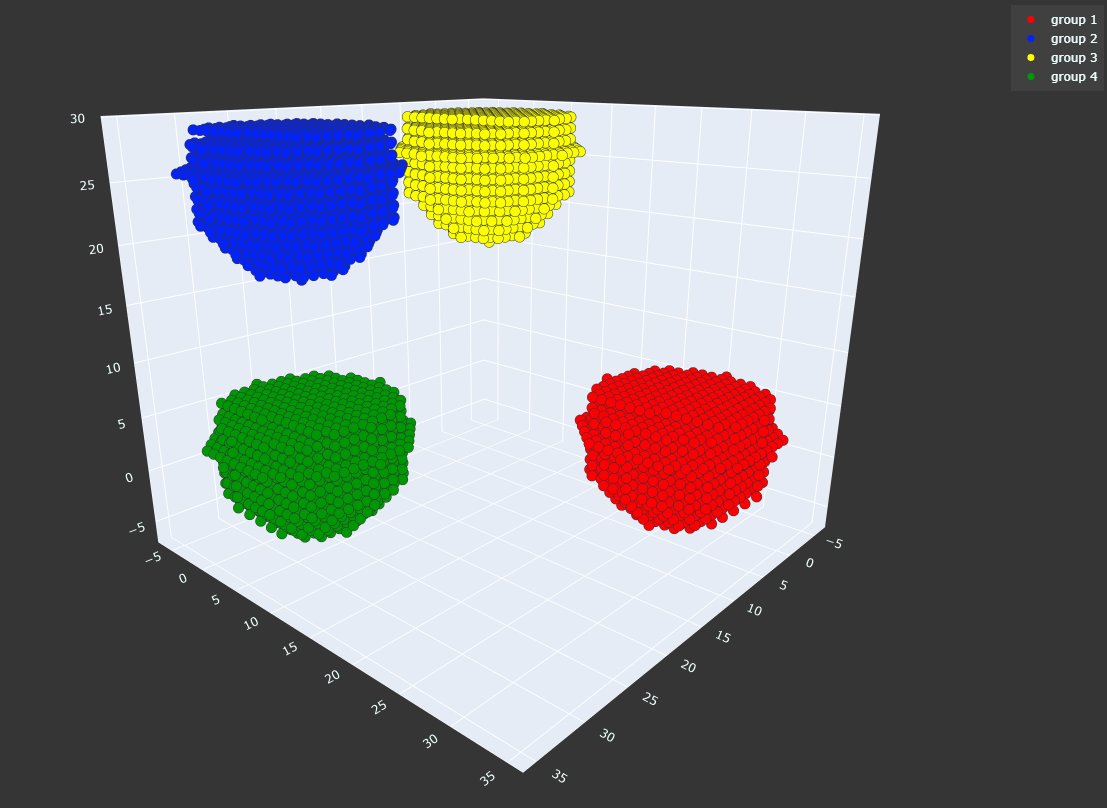
\includegraphics[width=0.75\linewidth]{images/groups.png}
    \caption{Network containing 4 groups with 2000 nodes per group}
    \label{fig:groups}
\end{figure}

To distribute the spheres in the coordinate system, it is first divided into cubes. Let $n_{max}$ be the number of nodes in the biggest group. To determine the side length $s$ of the cubes, it is necessary to know the radius $r$ of the smallest sphere that can fit $n_{max}$ nodes.

\subsection{Creating a sphere}
The nodes are placed only at coordinates $x,y,z \in \mathbb{N}$. To create a sphere that can fit $n_{max}$ nodes, the radius needs to be known before the exact coordinates are calculated. The problem with this is that the only way to get the exact radius for a sphere that can fit $n_{max}$ nodes that are all at coordinates $x,y,z \in \mathbb{N}$ is to use the algorithm depicted in \ref{alg:exact_radius}.
\begin{algorithm}
\caption{Calculating exact radius}
\label{alg:exact_radius}
\begin{algorithmic}
\Require {$(n_{max})$}
\Ensure {$r$}
\State $r \gets 0$
\State $n \gets 0$
\While{$n < n_{max}$}
    \State $r \gets r+1$
    \State coords $\gets$ calculate coordinates for all nodes in sphere with radius $r$
    \State $n \gets $ length of coords
\EndWhile
\end{algorithmic}
\end{algorithm}
This algorithm is inefficient because it computes all spheres until $r$ is big enough. This can be improved by estimating the number of nodes in a sphere of radius $r$ instead of computing the exact number. The number of nodes is estimated using the formula \ref{eq:sphere_lattice}.
\begin{equation}
\label{eq:sphere_lattice}
    \dfrac{4 \cdot \pi \cdot r^3}{3}
\end{equation}
This estimation incurs an error. \ref{eq:gauss_error} shows the best currently known formula for calculating this error which was discovered and proven by Zheng \cite{gaussSphereProblem}.
\begin{equation}
\label{eq:gauss_error}
    \sum_{\substack{x \in z^3 \\ |x| \leq r}}{P(x)} = O_{\epsilon, P}(r^{v + 84 / 63 + \epsilon})
\end{equation}
The true error bound is suspected to be $O_\epsilon(R^{1 + \epsilon})$ but this is currently not possible to prove. For the context of this work the simpler estimation shown in formula \ref{eq:gauss_error_rough} is sufficient.
\begin{equation}
\label{eq:gauss_error_rough}
    O_{\epsilon}(r^{21/16 + \epsilon})
\end{equation}

Let $r_e$ be the resulting radius required for $n_{max}$ nodes using the estimation. If $n_{max}$ is close to the boundary between two radii, then the resulting radius may be too large or too small due to the introduced error. For this reason, the resulting radius is decremented by one and the exact calculation is then used to find the correct required radius, as shown in algorithm \ref{alg:exact_radius_improved}. This will always find the smallest radius for a sphere containing at least $n_{max}$ points.

\begin{algorithm}
\caption{Calculating exact radius}
\label{alg:exact_radius_improved}
\begin{algorithmic}
\Require {$(n_{max})$}
\Ensure {$r$}
\State $r \gets 0$
\State $n \gets 0$
\While{$n < n_{max}$}
    \State $r \gets r + 1$
    \State $n \gets$ estimate amount of nodes in sphere with radius $r$
\EndWhile
\State $ r \gets r - 1$
\While{len(coords) $ < n_{max}$}
    \State coords $\gets$ calculate exact coords of nodes for radius $r$
\EndWhile
\end{algorithmic}
\end{algorithm}

The formula \ref{eq:sphere_inequality} represents the inequality for points inside or on the surface of a sphere centered at the origin in three-dimensional space, as proven by Gui and Moradifam \cite{sphereInequality}. A point is inside the sphere if this inequality is satisfied.
\begin{equation}
\label{eq:sphere_inequality}
    x^2 + y^2 + z^2 \leq r^2
\end{equation}
This means the bigger one of the values $x,y,z$ becomes, the smaller the other must be to satisfy the inequality. Using this knowledge, it is possible to construct an algorithm (shown in \ref{alg:calc_sphere_points}) that efficiently computes all triples of $x,y,z$ values that satisfy the inequality. The order of $z,x,y$ in the algorithm is important, so a half full sphere creates points that fill the sphere from the bottom to the top.
Starting with $z$ and $y=0$, transforming the formula to $x$ results in $|x| \leq \sqrt{(r^2 - z^2)}$, which corresponds to all possible values of $x$ with respect to $z$ and $r$. This range corresponds to $-a,a$ in the algorithm. Solving for $y$ then results in $|y| \leq \sqrt{(r^2 - z^2 - x^2)}$, which yields all possible values for $y$ with respect to $x,z,r$. This coincides with $-b,b$ in the algorithm.

\begin{algorithm}
\caption{Calculating lattice points}
\label{alg:calc_sphere_points}
\begin{algorithmic}
\Require {$r$}
\Ensure {$coords$}
\State $coords \gets []$
\For {$z := -r$ to $r$}
    \State $a \gets \lfloor\sqrt{(r^2 - z^2)}\rfloor$
    \For {$x := -a$ to $a$}
        \State $b \gets \lfloor\sqrt{(a^2 - x^2)}\rfloor$
        \For {$y := -b$ to $b$}
            \State coords $\gets (x,y,z)$
        \EndFor
    \EndFor
\EndFor
\end{algorithmic}
\end{algorithm}

The Python implementation of this function takes in an amount of points $n$ and returns a list of triples of length $n$ containing the resulting coordinates and the radius $r$ of the sphere.

\section{Arranging the spheres}
After calculating the coordinates and radii for each sphere (one for each group), the biggest radius $r_{max}$ is known. Using this, the side length of the cubes can be calculated. To create some space between the spheres, this side length $s$ is calculated as $s = 2 * r_{max} * 1.25$ to add an empty space of 12.5\% of the sphere diameter on each side.

The cubes are always created within a larger cube, e.g. the number of cubes is $c = x^3$. $x$ is the side length of the bigger cube in cubes (e.g. a side length of $x=3$ cubes results in $c=27$ smaller cubes). In order not to spread out the spheres unnecessarily, the smallest number of cubes should be created. The minimum required number of cubes is the number of spheres/groups. To get the next higher value for $c$, $x$ can be calculated by $x =\lceil\sqrt[3]{num\_groups}\rceil$.

Using this the algorithm \ref{alg:cube_offsets} computes the coordinates of bottom left corner of each cube.

\begin{algorithm}
\caption{Calculating cube offsets}
\label{alg:cube_offsets}
\begin{algorithmic}
\Require {$num\_group, r_{max}$}
\Ensure {$offsets$}
\State $s \gets \lceil 2 * r_{max} * 1.25\rceil$
\State $o \gets \lceil 2 * r_{max} * 0.125\rceil$
\State $c \gets \lceil\sqrt[3]{num\_groups}\rceil$
\For {$x,y,z := 0$ to $c$}
    \State offsets $\gets (x \cdot s + o, y \cdot s + o, z \cdot s + o)$
\EndFor
\end{algorithmic}
\end{algorithm}

For each sphere a random cube is selected and its offsets are added to the coordinates of all points within the sphere, resulting in the final coordinates for all nodes in the network.

\section{Creating the scatter graph}
\label{sub:scatter_graph}
In the final graph it must be possible to toggle the visibility of each group. To achieve this, the coordinates for each group are stored separately and only the active ones are added to the coordinate lists for the \texttt{Scatter3d} call.

\begin{lstlisting}[language=python, caption={Creation of the node trace}, label={lst:node_trace}]
for group in self.network.groups:
    if group.id not in self.hidden_groups:
        x, y, z = zip(*self.group_coords[group.id])
        aXn.extend(x)
        aYn.extend(y)
        aZn.extend(z)
        colors.extend([group.color] * len(x))
trace1 = go.Scatter3d(
    x=aXn,
    y=aYn,
    z=aZn,
    mode="markers",
    name="nodes",
    marker=dict(
        symbol="circle",
        size=6,
        color=colors,
        line=dict(color="rgb(50,50,50)", width=0.5),
    ),
    uirevision="0",
    showlegend=False,
)
\end{lstlisting}

The code in \ref{lst:node_trace} creates the trace that displays all active nodes. Whenever the visibility of a group is toggled, this trace must be rebuilt. It is important to note that the coordinates for the nodes in the x,y,z arrays contain the nodes in ascending order by their id. This means that nodes of group 0 come first starting with node 0, then group 1, and so on. This is important for creating color sequences based on the node states, which is discussed in section \ref{sec:color_sequence}.

\section{Displaying the edges}
The edges are displayed using a second \texttt{Scatter3d} with the \texttt{lines} mode. For this the x,y and z arrays need the format of [xStart, xEnd, None] for each line. This means that a coordinate array for 100 lines would have a length of 300.

The current format in which the edges are represented contains only the node ids that are connected by edges. This representation was created in section \ref{sub:havel_hakimi}. To translate these node ids to the coordinates of the nodes calculated in section \ref{sub:displayNodes}, a map is created when the coordinates are calculated for each node. This map stores the node id as a key and the index of its coordinates, in the coordinate array, as value. This map can be used to calculate the start and end coordinates for all edges of visible groups, which is done by looking up the coordinates of the start and end nodes by using their ids and the map. The python code that realizes this can be seen in listing \ref{lst:edge_creation}.
\begin{lstlisting}[language=python, caption={Creation of the edge coordinate arrays}, label={lst:edge_creation}]
 for edge in edges:
    _from, to = edge[0], edge[1]
    if not (_from in node_id_map and to in node_id_map):
        continue
    from_ind = node_id_map[_from]
    to_ind = node_id_map[to]
    aXe.extend([node_coords_x[from_ind], node_coords_x[to_ind], None])
    aYe.extend([node_coords_y[from_ind], node_coords_y[to_ind], None])
    aZe.extend([node_coords_z[from_ind], node_coords_z[to_ind], None])
\end{lstlisting}

The trace is then created using the \texttt{Scatter3d} call from listing \ref{lst:edge_trace}.
\begin{lstlisting}[language=python, caption={Creation of the edge trace}, label={lst:edge_trace}]
trace2 = go.Scatter3d(
            x=aXe,
            y=aYe,
            z=aZe,
            mode="lines",
            uirevision="0",
            line=dict(color="rgb(125,125,125)", width=1),
            hoverinfo="none",
            showlegend=False,
        )
    \end{lstlisting}

\chapter{Visual Simulation}
\label{cha:visual_simulation}
To simulate epidemics in a network, each node needs to store its state. As explained in %TODO ref
each node can have one of the following states: healthy, cured, infected, vaccinated, deceased. The current state is stored in the node along with the disease it is infected with for the state \texttt{infected}. The amount of cycles the node has been infected and the total amount of times the node has been infected are also stored. Each node also contains all nodes it is connected to.

Using this information the simulation can be done using the algorithm in \ref{alg:simulation}.

\begin{algorithm}
\caption{Simulate epidemics}
\label{alg:simulation}
\begin{algorithmic}
\Require {$nodes$}
\For{node in $nodes$}
    \If {node is not vaccinated}
        \State vaccinate according to vaccination chance of group
    \EndIf
    \If {node is infected}
        \If {infection time > disease duration}
            \State kill or cure node according to rates of disease
        \Else
            \State infection time $\gets$ infection time + 1
            \For{each connected node that is not infected}
                \State infect node according to rate of disease 
                \State (depending on vaccination status and previous infections)
            \EndFor
        \EndIf
    \EndIf
\EndFor
\end{algorithmic}
\end{algorithm}

\section{Displaying the status}
To display the current state of the simulation the nodes are colored according to their state. Each state has a configurable color with infected having different colors for each disease. Since nodes may have multiple concurrent states (eg. vaccinated and infected) each state has a priority and the color of the highest priority state will be displayed. A lower number means a higher priority.
\begin{enumerate}
    \item Infected/Deceased
    \item Vaccinated
    \item Healthy/Cured
\end{enumerate}

Using this priority list a sequence of colors can be generated from all node states. This sequence is created for the nodes in ascending order of their ids. This is important because the \texttt{Scatter3d} graph requires the colors in the same order as the coordinates which are also in ascending order as mentioned in section \ref{sub:scatter_graph}. The color of the graph can then be updated using the \texttt{update\_trace} method as seen in listing \ref{lst:update_color}

\begin{lstlisting}[language=python, caption={Updating the colors of the graph}, label={lst:update_color}]
fig.update_traces(selector=dict(name="nodes"), marker=dict(color=state_colors))
\end{lstlisting}

% \chapter{Introduction}
% \label{cha:introduction}
% \section{Motivation}
An epidemic outbreak can have a major impact on the world. Past epidemics have shown that
if we do not know how to counteract an epidemic outbreak and are not prepared for 
such cases, a new disease can cause the death of major parts of the world. The black
death caused the death of about 30\% to 60\% of all Europeans (75-200 million)
during the 1300s \cite{blackDeath}.
To better understand such scenarios simulations play an important role since studying real
cases of epidemic outbreaks is difficult as there are only so many in the history of humans.
Also it is important in case an outbreak happens to be able to simulate the next few days/weeks
to accurately predict how the epidemic will evolve.

For this reason this work will discuss an approach to simulate such epidemics by modeling
networks of persons and then simulating the spreading of diseases with different properties
in these networks.

\section{Problem definition}
A model of the social network the disease is spreading in is curcial to the simulation.
Depending on the transmission method of the disease this network can be highly connected in 
the case of a disease with airborne transmission or have only few connections for diseases
that are for example sexually transmitted. In addition to that different diseases can spread
completely different in the same social network even if the have the same transmission method
because the characteristics of the disease also play an important role in how it spreads. 
As suggested by Easley and Kleinberg \cite{networks}
the transmission of computer viruses works in a similar way an thus is also able to be modeled
by using networks.

The networks that can be created using the app must be able to model different social
networks. The important part for the epidemics simulation is the modeling of the amount
of contacts with other humans each human has. Since each group can contain a significant amount
of members an efficient method for creation networks with large amounts of nodes is required, which
still allows to model most social networks.

A method to visually display these networks in a clear way is required. The visual 
representation must still be usable with large amounts of nodes (eg. over 100,000 nodes).
To make the visualization of the network more usable some settings need to be provided
to alter the displayed network, like hiding certain connections or nodes. It also needs
ways to represent the current state of the network in respect to the spread of the diseases.

The app also needs to allow for creation of multiple diseases with different properties.
To simulate various epidemic scenarios properties like the infectiousness, duration of illnes
or fatality need to be editable. 

The app should be able to simulate multiple diseases at the same time. The simulation needs
to take into account which humans have contact with each other and then simulate the spreading
of the diseases according to the properties of each disease and group of humans.

During the simulation the app will collect statistics to allow a review of key information
after a simulation, like the amount of new infections over time.

% \chapter{Terminology}
% \label{cha:terminology}
% \input{tex/terminology}

% \chapter{Defining different types of Games}
% \label{cha:gameDefinitions}
% \input{tex/gameDefinitions}

% \chapter{Solution Strategies and Nash Equilibria}
% \label{cha:solutionStrategies}
% \input{tex/solutionStrategies}

% \chapter{Complexity of finding Nash equilibria}
% \label{cha:complexityOfFindingNash}
% \input{tex/complexityOfFindingNash}

% \chapter{Summary}
% \label{cha:summary}
% \section{Achieved Results}
In chapter \ref{cha:general_principles} the theory of epidemics was introduced. The two main parts of epidemics were discussed, networks and diseases. Three existing models and their respective limitations were explained, a simple tree-based model, the SIR Model and the SIS Model. These were  combined and extended to create the custom model used in this work. This custom model was explained in detail in section \ref{sec:custom_model}.

An app was created that uses the custom model to allow for simulations of epidemics. The app includes functions for modeling social networks, creating diseases, running simulations with the created networks and diseases and collecting statistics about the simulation. The general functionality of the app has been outlined in chapter \ref{cha:implementation} and its implementation is described in chapters \ref{cha:network_generation}, \ref{cha:network_display} and \ref{cha:visual_simulation}, which explain the process and algorithms involved in creating the app.

After creating the app some experiments were conducted to support the theories discussed in chapter \ref{cha:general_principles}. These experiments were performed using the developed app. The results of the simulations coincided with the theories of how the diseases are expected to behave. This indicated the importance of factors like the reproductive number $R_0$ in epidemics. The findings of these experiments and theories can be used to better prepare for real-world scenarios of epidemics. They help to understand the behavior of diseases and their lifetime in complex social networks.

\section{Outlook}
\subsection{Extensibility of the Results}
The network editor can be extended to allow precise control over which nodes are connected to which. This requires a solution that still allows fast creation of large networks while providing such fine control over the connections.

For very large networks, the computation can take a long time. Tests showed that networks with \~100,000 nodes took almost 30 minutes to generate. A big factor for this long time is that Python is an interpreted language, which makes such calculations relatively slow compared to the same calculations in a compiled language like C++. The app could be reimplemented in C++ which would reduce the computing time, but since C++ does not provide a package like plotly, a custom implementation for displaying the graphs is necessary, which can be time consuming to implement.

\subsection{Transferability of the Results}
The results achieved using the simulation can be applied to real-world scenarios. These simulations can help to predict how an epidemic will evolve over time. This can be used to test how certain factors affect the spreading of the disease to determine what countermeasures are necessary to suppress the disease and ensure the safety of the population. One example might be reducing the number of connections in the network, which could be achieved in the real world by implementing social distancing measures. Another factor that can be tested is whether a vaccine that reduces the infection probability by a certain amount is sufficient to make the disease die out or what percentage of people would need to be vaccinated to achieve this.

Without tools to simulate the behavior of diseases, it is almost impossible to predict what will happen, making it difficult to decide on the necessary countermeasure until it might be too late. This is why tools for simulation are necessary in the field of epidemics.


%-----------------------------------------------------------------------
\appendix

%---
\printbibliography[heading=bibintoc]

\end{document}